% PREAMBLE
\documentclass[11pt]{amsart}
\usepackage[T1]{fontenc}
\usepackage{lmodern}
\usepackage{microtype}
\usepackage{amsmath,amssymb}
\usepackage{mathtools}
\usepackage{graphicx}
\usepackage{booktabs}
\usepackage{tikz}
\usepackage[colorlinks=true,linkcolor=blue!45!black,citecolor=blue!45!black,urlcolor=blue!45!black]{hyperref}
\usepackage[capitalize]{cleveref}

\newtheorem{theorem}{Theorem}[section]
\newtheorem{proposition}[theorem]{Proposition}
\newtheorem{lemma}[theorem]{Lemma}
\newtheorem{corollary}[theorem]{Corollary}
\newtheorem{conjecture}[theorem]{Conjecture}
\theoremstyle{definition}
\newtheorem{definition}[theorem]{Definition}
\newtheorem{fact}[theorem]{Fact}
\theoremstyle{remark}
\newtheorem{remark}[theorem]{Remark}

\title[Order Sensitivity of Kronecker Design Words]{Order Sensitivity of Kronecker Design Words: What the Perfect Shuffle Cannot See}
\author{Carlo Mitchener}
\address{MrlyProd, Inc.}
\email{carlo.mitchener@gmail.com}
\date{First published 2026-08-23, revised 2026-09-03}

% PAPER
\begin{document}

\begin{abstract}
Nest one small black-and-white pattern inside another, then swap the order of the nesting. The picture keeps its size and its number of black cells, but it can fall apart into twice as many pieces. The algebraic half is classical: the two orders differ by a perfect shuffle, so fill, rank, spectrum and trace cannot see the order. A shuffle does not preserve which cells touch, so connectivity, holes and perimeter are free to change, and they do. We give the smallest two-cell witness, a classification of the two-cell designs, a census of nine observables over all $225$ two-letter and $1000$ three-letter words in stated alphabets, and a rank-$4$ linear representation of the component count, exact on every word of length at most four. An earlier claim that no such representation exists is retracted here, with its date. Why the rank is $4$ is open, and is this paper's largest debt.
\end{abstract}

% TITLE PAGE
\makeatletter
\global\let\titledate\@date
\global\let\paperabstract\@setabstracta
\global\let\@date\@empty
\global\let\@setabstract\relax
\makeatother

\maketitle

\begin{center}
\normalfont\footnotesize\titledate
\end{center}

\vspace*{\stretch{1}}

\begin{center}

\includegraphics[width=0.5\textwidth]{figures/avatar.png}
\end{center}

\vspace*{\stretch{1.25}}

\newpage

\paperabstract

% BODY
\section{Introduction}
\label{sec:intro}

Take a two-by-two square and colour some of its four cells black. That is a \emph{design}. Now substitute a shrunken copy of a second design into every black cell of the first: a four-by-four picture. Do it the other way round --- second design outside, first inside --- and you get a different picture with exactly the same number of black cells.

\Cref{fig:witness} is the smallest interesting instance. Both pictures have four black cells in a four-by-four frame. One is four separate specks. The other is two dominoes. The order of nesting decided which.

\begin{figure}[!ht]
\centering
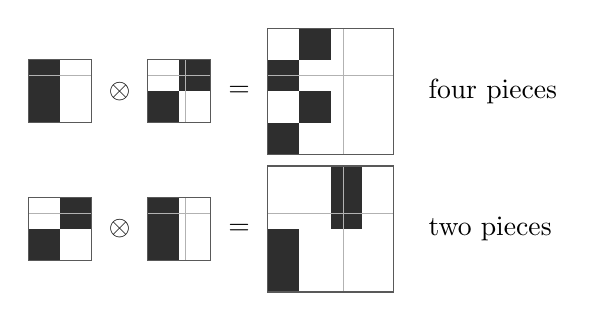
\begin{tikzpicture}[x=4mm,y=4mm]
  \begin{scope}[yshift=1.75cm]
    \fill[black!82] (0,1) rectangle ++(1,1);
    \fill[black!82] (0,2) rectangle ++(1,1);
    \draw[black!30] (0,1) grid (2,3);
    \draw[black!65] (0,1) rectangle (2,3);
    \node at (2.9,2) {$\otimes$};
    \fill[black!82] (3.8,1) rectangle ++(1,1);
    \fill[black!82] (4.8,2) rectangle ++(1,1);
    \draw[black!30] (3.8,1) grid (5.8,3);
    \draw[black!65] (3.8,1) rectangle (5.8,3);
    \node at (6.7,2) {$=$};
    \fill[black!82] (7.6,0) rectangle ++(1,1);
    \fill[black!82] (7.6,2) rectangle ++(1,1);
    \fill[black!82] (8.6,1) rectangle ++(1,1);
    \fill[black!82] (8.6,3) rectangle ++(1,1);
    \draw[black!30] (7.6,0) grid (11.6,4);
    \draw[black!65] (7.6,0) rectangle (11.6,4);
    \node[anchor=west] at (12.4,2) {four pieces};
  \end{scope}
  \begin{scope}
    \fill[black!82] (0,1) rectangle ++(1,1);
    \fill[black!82] (1,2) rectangle ++(1,1);
    \draw[black!30] (0,1) grid (2,3);
    \draw[black!65] (0,1) rectangle (2,3);
    \node at (2.9,2) {$\otimes$};
    \fill[black!82] (3.8,1) rectangle ++(1,1);
    \fill[black!82] (3.8,2) rectangle ++(1,1);
    \draw[black!30] (3.8,1) grid (5.8,3);
    \draw[black!65] (3.8,1) rectangle (5.8,3);
    \node at (6.7,2) {$=$};
    \fill[black!82] (7.6,0) rectangle ++(1,1);
    \fill[black!82] (7.6,1) rectangle ++(1,1);
    \fill[black!82] (9.6,2) rectangle ++(1,1);
    \fill[black!82] (9.6,3) rectangle ++(1,1);
    \draw[black!30] (7.6,0) grid (11.6,4);
    \draw[black!65] (7.6,0) rectangle (11.6,4);
    \node[anchor=west] at (12.4,2) {two pieces};
  \end{scope}
\end{tikzpicture}
\caption{The same two designs in both orders. Domino outside, anti-diagonal pair inside: four isolated cells. The other way round: two dominoes. Four black cells either way.}
\label{fig:witness}
\end{figure}

Nesting is the Kronecker product. A design is a subset of the four corners of $\{0,1\}^2$, so there are $16$ of them and we index them by the $4$-bit code $c$. A word $w=(c_1,\dots,c_L)$ of design codes gives the $2^L \times 2^L$ binary array
\[
  A_w \;=\; A_{c_1} \otimes A_{c_2} \otimes \cdots \otimes A_{c_L},
\]
outermost factor first. Call an observable of $A_w$ \emph{order-blind} if it depends only on the multiset $\{c_1,\dots,c_L\}$, and \emph{order-sensitive} otherwise. \Cref{fig:witness} says the number of connected components is order-sensitive. Which observables join it?

Half of that question has a classical answer, and it is worth stating first because it decides the shape of everything else. For square matrices $A$ and $B$ there is a permutation matrix $S$, the perfect shuffle or commutation matrix, with $B \otimes A = S\,(A \otimes B)\,S^{\mathsf T}$; see Henderson and Searle~\cite{hendersonsearle} and Van Loan~\cite{vanloan}. The two orders differ by relabelling rows and columns by the \emph{same} permutation. Every functional of a square array that survives such a relabelling is therefore order-blind for free: the side length, the number of black cells, the density, the rank, the characteristic polynomial, the determinant, and the trace. The count of black cells on the main diagonal \emph{is} the trace. Nothing in that list is news, and none of it is this paper's.

What is this paper's is the other half. The shuffle permutation moves cells around; it does not preserve which cells are next to which. Pixel adjacency --- the relation ``these two black cells share an edge'' --- is not shuffle-invariant. That single sentence is the dividing line. Everything on the algebraic side of it is order-blind by \cref{prop:shuffle}; everything on the geometric side is free to break, and the content of this paper is which parts break, how early, and how far.

The answers, in order. Connected components break immediately, and \cref{fig:witness} is the lexicographically first witness among the two-cell designs (\cref{thm:witness}). Among the six two-cell designs the behaviour is completely classified: connected pairs commute with connected pairs, diagonal pairs commute with diagonal pairs, and a connected pair against a diagonal pair \emph{never} commutes, always giving four against two (\cref{thm:dichotomy}). Above two cells everything collapses to a single component in both orders (\cref{thm:kthree}). The boundary cell count is order-blind at length two for all $256$ ordered code pairs, by an exact pairing of the only four cells that can be interior (\cref{thm:boundary}), and becomes order-sensitive at length three. An exhaustive census (\cref{fact:landscape}) counts, observable by observable, how many multisets actually split.

Then the part that surprised us. The component count of $A_w$ grows without bound --- it reaches $2 \cdot 4^{L-1}$ at length $L$ (\cref{prop:peak}) --- and the natural geometric bookkeeping needed to compute it grows without bound too (\cref{prop:kappa}). Nevertheless the map $w \mapsto \operatorname{comp}(A_w)$ is a rational series of rank $4$: six explicit integer matrices, one per design class, reproduce the component count of every one of the $54{,}241$ words of length at most four as a single matrix product (\cref{fact:cocycle}). By the Schützenberger theory of rational series~\cite{schutzenberger,berstelreutenauer} a finite Hankel rank is exactly a finite linear representation; that theorem is theirs, and only the matrices are ours. We do not know why the rank is $4$. \Cref{sec:repro} states that as the paper's open problem and its largest debt.

An earlier version of this work asserted the opposite --- that no finite-state description of the component count exists. That claim is wrong and is retracted here in full (\cref{rem:retraction}), with the date and the reason. Publishing the retraction next to the result costs a paragraph and is the only thing that makes the surrounding numbers worth trusting.

\subsection*{What this is not}

Three neighbouring literatures answer questions that look like ours and are not.

\emph{Fractal squares.} Iterating a single design forever gives a self-similar limit set, and the topology of those limit sets --- how many connected components the \emph{limit} has --- is a developed subject~\cite{fractalsquares}. Our objects are the finite level-$L$ pictures, and a level-$L$ component count is not a statement about any limit; the two can disagree in both directions.

\emph{Non-autonomous iterated function systems.} An infinite aperiodic word of designs is precisely a non-autonomous IFS, and that literature owns the limiting object, its dimension and its topology~\cite{nonautoifs,nonautotop}. We own the finite-level combinatorics that sits underneath. \Cref{cor:block} explains the boundary between the two: every \emph{periodic} word collapses by associativity to the stationary self-similar theory of its one-period composite tile, so periodicity buys nothing new, and genuinely non-stationary behaviour requires an aperiodic word.

\emph{Graph tensor products.} Weichsel's theorem~\cite{weichsel} decides when the tensor product of two connected graphs is connected, and Kronecker graph models~\cite{kroneckergraphs} build large networks by exactly the operation in our title. Neither applies here. In a graph tensor product two vertices are adjacent when their coordinates are adjacent in both factors; in our pictures two cells are adjacent when they share an edge of the grid, which mixes the factors through carrying. The two adjacency relations are different, and so are the answers.

\section{Definitions}
\label{sec:def}

Throughout, base $2$ and dimension $2$ are fixed.

\begin{definition}[Designs and words]
\label{def:design}
A \emph{design} is a code $c \in \{0,1,\dots,15\}$, encoding the set of filled corners
\[
  F_c \;=\; \bigl\{(i,j) \in \{0,1\}^2 \;:\; \lfloor c/2^{\,i+2j} \rfloor \text{ is odd}\bigr\},
  \qquad k(c) = |F_c|,
\]
and $A_c$ is the $2 \times 2$ binary array with $A_c[i][j] = 1$ exactly when $(i,j) \in F_c$. Rows are indexed downward from $0$ and columns rightward from $0$. Thus $A_3$ is the left column, $A_5$ the top row, $A_6$ the anti-diagonal pair $\{(1,0),(0,1)\}$, $A_9$ the main diagonal, and $A_{15}$ the full tile. For a word $w = (c_1,\dots,c_L)$ of design codes the \emph{mixed product} is the $2^L \times 2^L$ binary array $A_w = A_{c_1} \otimes \cdots \otimes A_{c_L}$, with $A_{\varepsilon}$ the $1 \times 1$ array $(1)$ for the empty word. Its fill is $\prod_i k(c_i)$.
\end{definition}

Concretely, cell $(x,y)$ of $A_w$ is filled exactly when $(x_j, y_j) \in F_{c_j}$ for every $j$, where $x_j$ and $y_j$ are the $j$-th binary digits of $x$ and $y$ counted from the most significant. The first letter of the word is the outermost, coarsest factor.

\begin{definition}[Order-blind and order-sensitive]
\label{def:blind}
Two words are \emph{multiset-equivalent} if one is a permutation of the other. An observable $\phi$ is \emph{order-blind at length $L$} on a set of codes if $\phi(A_w)$ agrees on all multiset-equivalent words of that length, and \emph{order-sensitive} otherwise. A multiset is \emph{counted} in a census only if it admits two or more distinct orderings; a constant word cannot exhibit order sensitivity.
\end{definition}

The observables are fixed once and used with these meanings everywhere below. The conventions matter: two of them can be read another way, and the other reading inverts the answer.

\begin{definition}[Observables]
\label{def:obs}
Let $X$ be an $n \times n$ binary array.
\begin{itemize}
\item $\operatorname{comp}(X)$ is the number of \emph{$4$-connected} components of the filled cells.
\item A filled cell is \emph{interior} if all four of its edge-neighbours exist in the grid and are filled. The \emph{boundary cell count} is $\operatorname{bd}(X) = \operatorname{fill}(X) - \operatorname{interior}(X)$. It counts cells.
\item The \emph{perimeter} $\operatorname{per}(X)$ is the number of exposed unit edges: $4\operatorname{fill}(X)$ minus twice the number of edge-adjacent filled pairs. It counts edges, not cells.
\item $\operatorname{holes}(X)$ is the number of $4$-connected components of the empty cells that do not meet the border of the grid.
\item $\chi(X) = \operatorname{comp}(X) - e_8(X)$, where $e_8(X)$ is the number of \emph{$8$-connected} components of the empty cells that do not meet the border. This is the Euler characteristic in the standard mixed-connectivity convention, in which $4$-connected foreground is paired with $8$-connected background.
\item $\operatorname{diag}(X)$ is the number of filled cells $(d,d)$, that is, the trace. $\operatorname{anti}(X)$ is the number of filled cells $(d, n-1-d)$. The \emph{anti-diagonal profile} is the vector of length $2n-1$ whose $s$-th entry is the number of filled cells $(x,y)$ with $x+y=s$.
\item $h(X)$ counts the rows in which both the leftmost and the rightmost cell are filled; $v(X)$ counts the columns in which both the top and the bottom cell are filled. These are the \emph{contact counts}: two side-by-side copies of $X$ touch exactly when $h(X)>0$, and two stacked copies touch exactly when $v(X)>0$.
\end{itemize}
\end{definition}

\begin{remark}[Two conventions that invert answers]
\label{rem:guards}
First, \emph{diagonal count} is not \emph{diagonal profile}. The trace is order-blind at every length (\cref{cor:algebraic}); the full anti-diagonal profile is order-sensitive already at length two, on $99$ of the $105$ eligible multisets, with the two one-cell designs $c=1$ and $c=2$ as the lexicographically first witness (\cref{fact:guards}). Read the profile where the count is meant and the theorem reverses.

Second, \emph{boundary cells} are not \emph{perimeter}. \Cref{thm:boundary} is about $\operatorname{bd}$, the cell count, and it is order-blind at length two. The perimeter is order-sensitive at length two, on $78$ of the $105$ multisets; the lexicographically first witness is the multiset $\{1,3\}$, whose two orders have perimeter $6$ and $8$ while both have boundary cell count $2$. Both numbers appear in \cref{fact:guards} so that neither reading can be taken by accident.

Third, $\chi$ and $\operatorname{holes}$ use \emph{different} background connectivity by design, so $\chi \neq \operatorname{comp} - \operatorname{holes}$ in general. It fails on exactly $10$ of the $225$ length-two words and $168$ of the $1000$ length-three words in the domains of \cref{fact:landscape}. The two columns of that table are not redundant and must not be subtracted from one another.
\end{remark}

Two alphabets are used. The \emph{full alphabet} is the $15$ non-empty codes $\{1,\dots,15\}$. The \emph{ten-code library} is $\{3,5,6,7,9,10,11,12,13,14\}$, the codes with $k(c) \in \{2,3\}$: the four one-cell designs and the full tile are excluded. Every census below names which alphabet it uses.

\section{Results}
\label{sec:res}

\subsection{The classical half}

\begin{proposition}[Perfect shuffle]
\label{prop:shuffle}
Let $A$ be $m \times m$ and $B$ be $n \times n$. There is a permutation matrix $S$ of size $mn$, depending only on $m$ and $n$, with $B \otimes A = S\,(A \otimes B)\,S^{\mathsf T}$. Consequently, if $\phi$ is any function of a square array with $\phi(P X P^{\mathsf T}) = \phi(X)$ for every permutation matrix $P$, then $\phi(A_w)$ is order-blind at every length.
\end{proposition}

\begin{corollary}
\label{cor:algebraic}
Side, fill, density, rank, characteristic polynomial, determinant and trace are order-blind at every word length. In particular the main-diagonal count satisfies
\[
  \operatorname{diag}(A_w) \;=\; \prod_{j=1}^{L} \bigl|\{d \in \{0,1\} : (d,d) \in F_{c_j}\}\bigr|,
\]
which is a product and therefore order-blind. Checked directly on all $15^3 = 3375$ words of length three over the full alphabet, zero mismatches.
\end{corollary}

\Cref{prop:shuffle} is classical~\cite{hendersonsearle,vanloan} and we reprint its one-line proof only so the paper stands alone. It is stated first because it fences off the entire algebraic side of the question. What follows is about observables that are \emph{not} invariant under simultaneous row and column permutation.

\subsection{Contact, boundary, and the two-cell classification}

\begin{lemma}[Contact law]
\label{lem:contact}
$h(A_w) = \prod_{j} h(A_{c_j})$ and $v(A_w) = \prod_{j} v(A_{c_j})$. In particular whether two adjacent copies of $A_w$ touch is order-blind and is decided factor by factor. Checked on all $3375$ words of length three, zero mismatches.
\end{lemma}

\begin{theorem}[Boundary cells are order-blind at length two]
\label{thm:boundary}
For all codes $a, b \in \{0,\dots,15\}$, $\operatorname{bd}(A_a \otimes A_b) = \operatorname{bd}(A_b \otimes A_a)$. Moreover, writing $S(p) = \{0,1\}^2 \setminus \{p\}$ and $\bar p = (1-p_1, 1-p_2)$,
\[
  \operatorname{interior}(A_a \otimes A_b) \;=\; \sum_{p \in \{0,1\}^2} \mathbf{1}\bigl[S(p) \subseteq F_a\bigr]\,\mathbf{1}\bigl[S(\bar p) \subseteq F_b\bigr],
\]
which is symmetric in $a$ and $b$ because $p \mapsto \bar p$ is an involution. Both the symmetry and the formula were checked on all $256$ ordered code pairs, zero mismatches.
\end{theorem}

\begin{theorem}[Components are order-sensitive]
\label{thm:witness}
$\operatorname{comp}(A_3 \otimes A_6) = 4$ and $\operatorname{comp}(A_6 \otimes A_3) = 2$. Among the six two-cell designs $\{3,5,6,9,10,12\}$, the pair $\{3,6\}$ is the lexicographically first that fails to commute.
\end{theorem}

\begin{theorem}[The two-cell dichotomy]
\label{thm:dichotomy}
Call a two-cell design \emph{adjacent} if its two cells share an edge (codes $3, 5, 10, 12$) and \emph{diagonal} otherwise (codes $6, 9$). For the component count:
\begin{enumerate}
\item adjacent against adjacent always commutes, giving $1$ if the two dominoes have the same orientation and $2$ if not;
\item diagonal against diagonal always commutes, giving $4$;
\item adjacent against diagonal \emph{never} commutes: $\operatorname{comp}(A \otimes D) = 4$ and $\operatorname{comp}(D \otimes A) = 2$ for every one of the eight ordered pairs.
\end{enumerate}
\end{theorem}

\begin{theorem}[Three cells or more]
\label{thm:kthree}
If $k(a) \ge 3$ and $k(b) \ge 3$ then
\[
  \operatorname{comp}(A_a \otimes A_b) = \operatorname{comp}(A_b \otimes A_a) = 1 .
\]
All $25$ ordered pairs from $\{7,11,13,14,15\}$ were checked, zero deviations.
\end{theorem}

\begin{corollary}[Block reduction: periodicity buys nothing]
\label{cor:block}
For any designs $c_1,\dots,c_p$ and any $L \ge 1$, associativity of the Kronecker product gives
\[
  \bigl(A_{c_1} \otimes \cdots \otimes A_{c_p}\bigr)^{\otimes L} \;=\; A_{u^L}, \qquad u = (c_1,\dots,c_p),
\]
as arrays, cell for cell. Hence every periodic word of period $p$ is the stationary self-similar picture of its one-period composite tile, a design at base $2^p$ with fill $\prod_i k(c_i)$, and every observable of a periodic word is governed by the ordinary one-tile theory. Genuinely non-stationary behaviour requires an aperiodic word. Checked cell for cell on all $225$ two-letter blocks at periods two and three.
\end{corollary}

\subsection{The census}

\begin{fact}[The order-sensitivity landscape]
\label{fact:landscape}
Over the full alphabet at length two there are $225$ words and $120$ multisets, of which $105$ admit two or more orderings. Over the ten-code library at length three there are $1000$ words and $220$ multisets, of which $210$ admit two or more orderings. The number of eligible multisets on which each observable of \cref{def:obs} takes two or more values is:

\begin{center}
\small
\begin{tabular}{lcc}
\toprule
Observable & length $2$, full alphabet & length $3$, ten-code library \\
\midrule
Fill, side, density & $0 / 105$ & $0 / 210$ \\
Main-diagonal count & $0 / 105$ & $0 / 210$ \\
Anti-diagonal count & $0 / 105$ & $0 / 210$ \\
Boundary cell count & $0 / 105$ & $36 / 210$ \\
Perimeter & $78 / 105$ & $188 / 210$ \\
Connected components & $74 / 105$ & $188 / 210$ \\
Euler characteristic & $78 / 105$ & $188 / 210$ \\
Holes & $10 / 105$ & $100 / 210$ \\
Anti-diagonal profile & $99 / 105$ & $204 / 210$ \\
\bottomrule
\end{tabular}
\end{center}

Checked by \texttt{scripts/verify.py} on exactly these two domains.
\end{fact}

\begin{fact}[The two scope guards and the connectivity clash]
\label{fact:guards}
On the length-two domain of \cref{fact:landscape}: the anti-diagonal profile is order-sensitive on $99$ of the $105$ eligible multisets, the lexicographically first witness being $\{1,2\}$ with profiles $(0,1,0,0,0,0,0)$ and $(0,0,1,0,0,0,0)$, while the anti-diagonal \emph{count} is order-blind on all $105$; the perimeter is order-sensitive on $78$ of the $105$, the lexicographically first witness being $\{1,3\}$ with perimeters $6$ and $8$, while both orders have boundary cell count $2$. Here the eligible multisets are ordered lexicographically as sorted pairs, and both minimality claims are by exhaustion over all earlier pairs. Furthermore $\chi \neq \operatorname{comp} - \operatorname{holes}$ on exactly $10$ of the $225$ length-two words and on exactly $168$ of the $1000$ length-three words. Checked by \texttt{scripts/verify.py}.
\end{fact}

\subsection{Growth, and a rank-\texorpdfstring{$4$}{4} representation}

\begin{proposition}[The component count grows like $4^L$]
\label{prop:peak}
For every $L \ge 1$, $\operatorname{comp}\bigl(A_{(15^{L-1}, 6)}\bigr) = 2 \cdot 4^{L-1}$. Over the full alphabet this is the exact maximum at lengths $1$ through $4$: the largest component counts are $2$, $8$, $32$, $128$, verified exhaustively over all $15^L$ words.
\end{proposition}

\begin{proposition}[The naive geometric state is unbounded]
\label{prop:kappa}
Let $\kappa(X)$ be the number of $4$-connected components of $X$ that meet the border of the grid. A component that meets no border cell cannot merge with anything outside $X$, so $\kappa$ counts the components whose fate is still undecided when $X$ is placed inside a larger picture, and bounds from above the number that can actually merge. Then $\kappa\bigl(A_{(15^{L-1},3)}\bigr) = 2^{L-1}$, so $\kappa$ is unbounded. Verified for $L = 1,\dots,7$.
\end{proposition}

So both the answer and the obvious way of computing it grow without bound. They are nevertheless produced by four numbers.

\begin{fact}[The component cocycle]
\label{fact:cocycle}
Let $\lambda = (1,0,0,0)$, $\gamma = (1,1,1,1)^{\mathsf T}$, and assign to each code the integer matrix of its class:
\[
M_{\{1,2,4,8\}} = \begin{pmatrix} 1&0&0&0 \\ 2&0&0&0 \\ 2&0&0&0 \\ 4&0&0&0 \end{pmatrix}\!,
\qquad
M_{\{6,9\}} = \begin{pmatrix} 2&0&0&0 \\ 4&0&0&0 \\ 4&0&0&0 \\ 8&0&0&0 \end{pmatrix}\!,
\]
\[
M_{\{3,12\}} = \begin{pmatrix} 0&1&0&0 \\ -2&3&0&0 \\ 0&2&0&0 \\ -4&6&0&0 \end{pmatrix}\!,
\qquad
M_{\{5,10\}} = \begin{pmatrix} 0&0&1&0 \\ 0&0&2&0 \\ -2&0&3&0 \\ -4&0&6&0 \end{pmatrix}\!,
\]
\[
M_{\{7,11,13,14\}} = \begin{pmatrix} -1&1&1&0 \\ -4&3&2&0 \\ -4&2&3&0 \\ -8&4&4&1 \end{pmatrix}\!,
\qquad
M_{\{15\}} = \begin{pmatrix} 0&0&0&1 \\ 0&0&-2&3 \\ 0&-2&0&3 \\ 4&-6&-6&9 \end{pmatrix}\!.
\]
Then $\operatorname{comp}(A_w) = \lambda\,M_{c_1} M_{c_2} \cdots M_{c_L}\,\gamma$ for every one of the $54{,}241$ words $w$ of length at most $4$ over the full alphabet, including the empty word. Zero mismatches; checked by \texttt{scripts/verify.py}.
\end{fact}

\begin{fact}[Hankel ranks of the length-four truncation]
\label{fact:ranks}
Index a $241 \times 241$ integer matrix by the words of length at most $2$ over the full alphabet, with entry $(u,v)$ equal to $\phi(A_{uv})$. Its rank is $4$ for $\phi = \operatorname{comp}$, $4$ for $\phi = \chi$, $8$ for $\phi = \operatorname{bd}$, and $11$ for $\phi = \operatorname{holes}$. These are ranks of a truncation and are therefore lower bounds on the Hankel rank of the full series; only for $\operatorname{comp}$ do we exhibit matrices (\cref{fact:cocycle}). Checked by \texttt{scripts/verify.py}.
\end{fact}

\begin{proposition}[Noncommutation is necessary, not sufficient]
\label{prop:noncomm}
Among the $15$ unordered pairs of the six matrices of \cref{fact:cocycle}, exactly $14$ fail to commute; the single commuting pair is $\{1,2,4,8\}$ with $\{6,9\}$, and there $M_{\{6,9\}} = 2\,M_{\{1,2,4,8\}}$. If $\operatorname{comp}$ takes different values on $(a,b)$ and $(b,a)$ then $M_a M_b \neq M_b M_a$. The converse is false: $M_3 M_5 \neq M_5 M_3$ while $\operatorname{comp}(A_3 \otimes A_5) = \operatorname{comp}(A_5 \otimes A_3) = 2$, and $M_7 M_{15} \neq M_{15} M_7$ while $\operatorname{comp}(A_7 \otimes A_{15}) = \operatorname{comp}(A_{15} \otimes A_7) = 1$. Both exhibited pairs are noncommuting yet order-blind at length two. Order sensitivity requires $\lambda(M_a M_b - M_b M_a)\gamma \neq 0$, which is strictly stronger than $M_a M_b \neq M_b M_a$.
\end{proposition}

\begin{remark}[Retraction, 2026-08-22]
\label{rem:retraction}
An earlier version claimed that the component count of $A_w$ is \emph{not} a finite-state function of the word $w$. The evidence offered was that one candidate state --- the four-corner partition of the running product --- reproduces the counts at length two and fails at length three, because the cells that connect two copies need not be corners. That evidence is real and the conclusion drawn from it is wrong: one failed candidate state bounds nothing about the state space. \Cref{fact:cocycle} exhibits a rank-$4$ linear representation, so the claim is withdrawn. What survives from the original argument is \cref{prop:kappa}: the naive geometric bookkeeping is genuinely unbounded. Hankel rank is the dimension of the span of the residual functions $v \mapsto \phi(A_{uv})$, not the size of any geometric state, and the two have no reason to agree.
\end{remark}

\begin{conjecture}[The representation is exact at every length]
\label{con:cocycle}
For every word $w$ over the full alphabet, at every length, $\operatorname{comp}(A_w) = \lambda\,M_{c_1} \cdots M_{c_L}\,\gamma$. \emph{Evidence:} exhaustive agreement on all $54{,}241$ words of length at most $4$ (\cref{fact:cocycle}), across a range in which the count itself grows from $1$ to $128$; the six matrices were obtained by exact rational elimination on a Hankel basis, so no fitting slack remains. \emph{Failure mode:} the rank of a truncated Hankel matrix is a lower bound only. A geometric contact pattern that first appears at length $5$ or beyond would raise the true rank, and the four coordinates $\varepsilon, 3, 5, 15$ would then be an accident of small words rather than a basis.
\end{conjecture}

\begin{conjecture}[The sharp maximum]
\label{con:peak}
$\max_{|w| = L} \operatorname{comp}(A_w) = 2 \cdot 4^{L-1}$ for every $L \ge 1$. \emph{Evidence:} the family of \cref{prop:peak} attains it for all $L$, proved; exhaustive optimality at $L \le 4$. \emph{Failure mode:} a word mixing several disconnecting factors could in principle beat the single-disconnector family at some length beyond the exhaustive range; the exhaustion stops at $L=4$ because $15^5$ words of side $32$ leave the seconds-long budget of \texttt{scripts/verify.py}.
\end{conjecture}

\begin{conjecture}[Boundary cells break at three and stay broken]
\label{con:boundary}
The boundary cell count is order-sensitive at every length $L \ge 3$ over the ten-code library. \emph{Evidence:} $36$ of $210$ eligible multisets at $L=3$ (\cref{fact:landscape}); the pairing argument of \cref{thm:boundary} is specific to the four central cells of a $4 \times 4$ grid and has no analogue once interior cells can appear away from the centre. \emph{Failure mode:} the count $36$ is small relative to $210$, and no mechanism is offered for why it should persist; a cancellation at some larger length is not excluded by anything proved here.
\end{conjecture}

\section{Proofs}
\label{sec:proofs}

\begin{proof}[Proof of \cref{prop:shuffle}]
Index the rows of $A \otimes B$ by pairs $(i_A, i_B)$ via $i = n\,i_A + i_B$, and the rows of $B \otimes A$ by the same pairs via $i' = m\,i_B + i_A$, where $i_A$ ranges over $\{0,\dots,{m-1}\}$ and $i_B$ over $\{0,\dots,{n-1}\}$. By definition $(A \otimes B)[(i_A,i_B)][(j_A,j_B)] = A[i_A][j_A]\,B[i_B][j_B] = (B \otimes A)[(i_B,i_A)][(j_B,j_A)]$. Let $S$ be the permutation matrix of the map $(i_A,i_B) \mapsto (i_B,i_A)$ on the $mn$ index pairs. The displayed identity says exactly that $B \otimes A$ is obtained from $A \otimes B$ by applying $S$ to rows and the same $S$ to columns, that is $B \otimes A = S (A \otimes B) S^{\mathsf T}$. For the consequence, let $w$ and $w'$ be multiset-equivalent. Any permutation is a product of adjacent transpositions, and by associativity an adjacent transposition of two letters of $w$ is a shuffle of the corresponding two Kronecker factors, conjugated by the identity on the factors outside them --- itself a simultaneous row and column permutation of $A_w$. Composing, $A_{w'} = P A_w P^{\mathsf T}$ for some permutation matrix $P$, so $\phi(A_{w'}) = \phi(A_w)$.
\end{proof}

\begin{proof}[Proof of \cref{cor:algebraic}]
Side, fill, density, rank, characteristic polynomial and determinant are unchanged by $X \mapsto PXP^{\mathsf T}$, and so is the trace; apply \cref{prop:shuffle}. For the product formula, cell $(x,x)$ of $A_w$ is filled exactly when $(x_j,x_j) \in F_{c_j}$ for every digit position $j$, by \cref{def:design}. The digits $x_1,\dots,x_L$ range independently over $\{0,1\}$ as $x$ ranges over $\{0,\dots,2^L-1\}$, so the number of filled diagonal cells is the product over $j$ of the number of admissible digits $d$, namely $|\{d : (d,d) \in F_{c_j}\}|$.
\end{proof}

\begin{proof}[Proof of \cref{lem:contact}]
Column $0$ of $A \otimes B$ is column $0$ of the outer factor combined with column $0$ of the inner, so $L(A \otimes B) = L(A) \otimes L(B)$ as vectors; likewise the last column satisfies $R(A \otimes B) = R(A) \otimes R(B)$. The entrywise product of Kronecker products of vectors is the Kronecker product of the entrywise products, so
\[
  h(A \otimes B) = \bigl\langle R(A) \otimes R(B),\, L(A) \otimes L(B) \bigr\rangle = \bigl\langle R(A), L(A) \bigr\rangle \cdot \bigl\langle R(B), L(B) \bigr\rangle,
\]
which is $h(A)h(B)$. Induction on the number of factors gives the product over the whole word. The argument on rows gives $v$. The final sentence is immediate: a product of per-factor quantities does not see the order, and it is positive exactly when every factor is.
\end{proof}

\begin{proof}[Proof of \cref{thm:boundary}]
Write $A = A_a$, $B = A_b$, so $A \otimes B$ is $4 \times 4$. A cell can be interior only if both its coordinates lie in $\{1,2\}$, since a cell in row $0$ or $3$ or column $0$ or $3$ is missing a neighbour. So the only candidates are the four central cells, and we index them by $p \in \{0,1\}^2$ through $z(p) = (2-p_1,\, 2-p_2)$; this is a bijection onto $\{1,2\}^2$.

Decompose a cell $(x,y)$ of the $4 \times 4$ grid as outer index $(\lfloor x/2 \rfloor, \lfloor y/2 \rfloor)$ and inner index $(x \bmod 2, y \bmod 2)$, so the cell is filled iff the outer index lies in $F_A$ and the inner index lies in $F_B$. For $z(p)$ the outer index is $(1-p_1, 1-p_2) = \bar p$ and the inner index is $(p_1,p_2) = p$, because $\lfloor (2-p_i)/2 \rfloor = 1-p_i$ and $(2-p_i) \bmod 2 = p_i$ for $p_i \in \{0,1\}$.

Now take the two vertical neighbours of $z(p)$, in rows $1-p_1$ and $3-p_1$. Since $1-p_1 \in \{0,1\}$ and $3-p_1 \in \{2,3\}$, their outer row indices are $0$ and $1$ respectively, and both have inner row index $(1-p_1) \bmod 2 = 1-p_1 = \bar p_1$. Their column decomposition is that of $z(p)$, namely outer $\bar p_2$ and inner $p_2$. So both vertical neighbours are filled exactly when $(\bar p_1, p_2) \in F_B$ and both cells of column $\bar p_2$ of $A$ lie in $F_A$. Symmetrically, both horizontal neighbours are filled exactly when $(p_1, \bar p_2) \in F_B$ and both cells of row $\bar p_1$ of $A$ lie in $F_A$.

Collect the conditions. On $A$: $\bar p \in F_A$, all of column $\bar p_2$, and all of row $\bar p_1$. The union of the cell $\bar p$, the column $\bar p_2$ and the row $\bar p_1$ is precisely the set of cells whose row is $\bar p_1$ or whose column is $\bar p_2$, and the only cell of $\{0,1\}^2$ failing both is $(p_1,p_2) = p$. Hence the condition on $A$ is $S(p) \subseteq F_A$. On $B$: $p \in F_B$, $(\bar p_1, p_2) \in F_B$ and $(p_1, \bar p_2) \in F_B$; these are the three cells other than $\bar p$, so the condition on $B$ is $S(\bar p) \subseteq F_B$.

Summing the indicator over the four candidates gives the displayed formula. Swapping $a$ and $b$ replaces the $p$-th term by the $\bar p$-th, and $p \mapsto \bar p$ is a fixed-point-free involution of $\{0,1\}^2$, so the four terms are permuted and the sum is unchanged. Since $\operatorname{fill}$ is order-blind by \cref{cor:algebraic}, $\operatorname{bd} = \operatorname{fill} - \operatorname{interior}$ is order-blind at length two as well.
\end{proof}

\begin{proof}[Proof of \cref{thm:witness}]
$F_3 = \{(0,0),(1,0)\}$ and $F_6 = \{(1,0),(0,1)\}$. In $A_3 \otimes A_6$ the outer factor places copies of $A_6$ in blocks $(0,0)$ and $(1,0)$, and within each block $A_6$ fills the cells $(1,0)$ and $(0,1)$. The four filled cells of the $4 \times 4$ grid are therefore $(1,0), (0,1), (3,0), (2,1)$. No two of these differ by exactly one in one coordinate and zero in the other, so all four are isolated and $\operatorname{comp} = 4$. In $A_6 \otimes A_3$ the outer factor places copies of $A_3$ in blocks $(1,0)$ and $(0,1)$, giving filled cells $(2,0),(3,0)$ and $(0,2),(1,2)$: two vertical dominoes. The two blocks differ in both coordinates, hence are not edge-adjacent, so no merging is possible and $\operatorname{comp} = 2$. Lexicographic minimality among the six two-cell designs is by exhaustion over the $15$ unordered pairs, and $(3,5)$ --- the only earlier pair --- commutes by \cref{thm:dichotomy}(1).
\end{proof}

\begin{proof}[Proof of \cref{thm:dichotomy}]
First record the contact counts of the two-cell designs, read off \cref{def:obs}. A vertical domino ($3$ or $12$) occupies one column, so no row contains both its leftmost and rightmost cell: $h = 0$; and its single occupied column contains both the top and bottom cell: $v = 1$. A horizontal domino ($5$ or $10$) is the transpose: $h = 1$, $v = 0$. A diagonal pair ($6$ or $9$) has one cell in each row and each column, so $h = v = 0$.

Now the general mechanism at length two. In $A_a \otimes A_b$ the filled cells are the union, over $q \in F_a$, of a copy of $A_b$ placed in block $q$. Two copies in blocks $q, q'$ can merge only if the blocks are edge-adjacent, and then only through the shared edge: if they are side by side this happens exactly when $h(A_b) > 0$, and if they are stacked exactly when $v(A_b) > 0$, by the definition of the contact counts. Copies in non-adjacent blocks can never merge, since every cell of one is at distance at least two from every cell of the other in some coordinate.

Case 3. Let $A$ be adjacent and $D$ diagonal. In $A \otimes D$ the two blocks of $F_A$ are edge-adjacent, but $h(A_D) = v(A_D) = 0$, so the copies do not merge; and within one copy the two cells of $D$ are not edge-adjacent, so each copy contributes $2$. Total $4$. In $D \otimes A$ the two blocks of $F_D$ are not edge-adjacent, so no merging occurs, and each copy of the connected domino $A$ contributes $1$. Total $2$. This is the same in all four choices of $A$ and both choices of $D$, so all eight ordered pairs give $(4,2)$ and none commutes.

Case 1. Let $A$ and $B$ both be dominoes. The blocks of $F_A$ are side by side if $A$ is horizontal and stacked if $A$ is vertical. Each copy of $B$ is connected, contributing one component, and the two copies merge exactly when the shared-edge contact of $B$ is positive: $h(A_B) > 0$ iff $B$ is horizontal, $v(A_B) > 0$ iff $B$ is vertical. So $\operatorname{comp}(A \otimes B) = 1$ if $A$ and $B$ have the same orientation and $2$ otherwise. That condition is symmetric in $A$ and $B$, so the two orders agree.

Case 2. Let $D_1, D_2$ be diagonal. The two blocks of $F_{D_1}$ are not edge-adjacent, so no merging occurs, and each copy of $D_2$ contributes its two isolated cells. Total $4$, in either order.
\end{proof}

\begin{proof}[Proof of \cref{thm:kthree}]
Let $k(c) \ge 3$. Then $F_c$ omits at most one cell of $\{0,1\}^2$. Of the two rows $\{(0,0),(0,1)\}$ and $\{(1,0),(1,1)\}$, at most one meets the omitted cell, so at least one row lies entirely in $F_c$, giving $h(A_c) \ge 1$; the same argument on columns gives $v(A_c) \ge 1$. Also $A_c$ is connected: for $k = 4$ this is clear, and for $k = 3$ the three cells form an L, in which the corner cell shares an edge with each of the other two.

Now let $k(a), k(b) \ge 3$. In $A_a \otimes A_b$ each of the $k(a) \ge 3$ copies of $A_b$ is connected, so contributes one component. Take two cells of $F_a$ that are edge-adjacent; such a pair exists since $A_a$ is connected and has at least two cells. Their two copies of $A_b$ merge, because the relevant contact count of $A_b$ is positive by the previous paragraph. Since $A_a$ is connected under edge-adjacency, every pair of copies is joined by a chain of edge-adjacent blocks, each link of which merges. Hence all copies lie in one component and $\operatorname{comp}(A_a \otimes A_b) = 1$. The hypothesis is symmetric in $a$ and $b$, so the same holds for the reversed order.
\end{proof}

\begin{proof}[Proof of \cref{cor:block}]
Immediate from associativity of the Kronecker product: both sides are the $pL$-fold product $A_{c_1} \otimes \cdots \otimes A_{c_p} \otimes A_{c_1} \otimes \cdots$, bracketed differently. The composite tile $A_u$ is a $2^p \times 2^p$ binary array with $\prod_i k(c_i)$ filled cells, and $A_{u^L} = A_u^{\otimes L}$ is exactly the level-$L$ self-similar picture of that single tile at base $2^p$.
\end{proof}

\begin{proof}[Proof of \cref{prop:peak}]
$A_{15}$ is the full $2 \times 2$ tile, so $A_{15}^{\otimes (L-1)}$ is the full $2^{L-1} \times 2^{L-1}$ square, with $4^{L-1}$ filled cells, every pair of horizontally or vertically neighbouring cells being edge-adjacent. Tensoring on the right with $A_6$ places a copy of the anti-diagonal pair in each of those $4^{L-1}$ blocks. Within a copy the two cells are not edge-adjacent. Between two edge-adjacent blocks no merging occurs, because $h(A_6) = v(A_6) = 0$ (see the proof of \cref{thm:dichotomy}), and non-adjacent blocks never merge. Hence every one of the $2 \cdot 4^{L-1}$ filled cells is isolated. The maximality statement at $L \le 4$ is exhaustion over all $15^L$ words.
\end{proof}

\begin{proof}[Proof of \cref{prop:kappa}]
$A_{15}^{\otimes(L-1)}$ is the full $2^{L-1}$ square. Tensoring on the right with $A_3$, whose only filled cells are $(0,0)$ and $(1,0)$, fills cell $(x,y)$ of the $2^L$ square exactly when $y$ is even. The filled set is thus $2^{L-1}$ full-height columns, pairwise separated by an empty column, so they are $2^{L-1}$ distinct components. Each runs the full height of the grid, so each meets the top row and hence the border. Therefore $\kappa = 2^{L-1}$, which is unbounded.
\end{proof}

\begin{proof}[Proof of \cref{prop:noncomm}]
The count of $14$ noncommuting pairs out of $15$, the identification of the one commuting pair, and the identity $M_{\{6,9\}} = 2 M_{\{1,2,4,8\}}$ are finite computations on six integer matrices, performed and asserted in the script named in \cref{sec:repro}. For necessity, suppose $\operatorname{comp}$ differs on $(a,b)$ and $(b,a)$. By \cref{fact:cocycle} these values are $\lambda M_a M_b \gamma$ and $\lambda M_b M_a \gamma$, so $\lambda(M_aM_b - M_bM_a)\gamma \neq 0$ and in particular $M_aM_b \neq M_bM_a$. The two displayed counterexamples refute the converse: the matrix products differ, but the bilinear form $\lambda(\cdot)\gamma$ annihilates the commutator, and the direct component counts agree, both by \cref{thm:dichotomy}(1) for $\{3,5\}$ and by \cref{thm:kthree} for $\{7,15\}$. Hence noncommutation of the cocycle matrices is necessary for order sensitivity and not sufficient.
\end{proof}

\section{Reproducibility}
\label{sec:repro}

One script regenerates every number in this paper, \texttt{scripts/verify.py}: plain \texttt{python3}, standard library only, no arguments, no network, all paths relative. Run it from the lane root with \texttt{python3 scripts/verify.py}. It prints one line per check and \texttt{all green} at the end; every check is an assertion that names what it got and what it wanted, and any failure exits non-zero. Total runtime is about $4.5$ seconds on a laptop. A second script, \texttt{scripts/figure.py}, redraws the SVG figure embedded in the lane README and takes well under a second; the figure in this paper is drawn inline in Ti\emph{k}Z and needs no script.

What \texttt{scripts/verify.py} covers, in order, with its exact domains:

\begin{itemize}
\item \Cref{thm:witness}: the two counts $4$ and $2$, and lexicographic minimality by exhaustion over the $15$ unordered pairs of the six two-cell designs.
\item \Cref{thm:boundary}: boundary-cell symmetry and the interior formula, both on all $256$ ordered pairs $(a,b)$ with $a,b \in \{0,\dots,15\}$, including the empty design.
\item \Cref{cor:algebraic} and \cref{lem:contact}: the main-diagonal product formula and the two contact products, each on all $15^3 = 3375$ words of length three over the full alphabet.
\item \Cref{thm:dichotomy}: all $8$ adjacent-diagonal ordered pairs give $(4,2)$; all $16$ adjacent-adjacent ordered pairs commute; all $4$ diagonal-diagonal ordered pairs give $4$.
\item \Cref{thm:kthree}: all $25$ ordered pairs from $\{7,11,13,14,15\}$ give $1$.
\item \Cref{cor:block}: cell-for-cell equality for all $225$ two-letter blocks at periods two and three.
\item \Cref{fact:landscape}: the full census. Length two over the $15$ non-empty codes, all $225$ words, $120$ multisets, $105$ eligible. Length three over the ten-code library $\{3,5,6,7,9,10,11,12,13,14\}$, all $1000$ words, $220$ multisets, $210$ eligible. Nine observables each.
\item \Cref{fact:guards}: the profile witness $\{1,2\}$ and the perimeter witness $\{1,3\}$, each confirmed lexicographically first by scanning all $105$ eligible multisets in order, and the counts $10$ of $225$ and $168$ of $1000$ on which $\chi \neq \operatorname{comp} - \operatorname{holes}$.
\item \Cref{fact:cocycle}: the representation against directly computed component counts on all $54{,}241$ words of length at most four over the full alphabet, the empty word included.
\item \Cref{prop:peak}: $\operatorname{comp}(A_{(15^{L-1},6)}) = 2 \cdot 4^{L-1}$ for $L = 1,\dots,6$, and the exhaustive maxima $2, 8, 32, 128$ at $L = 1,\dots,4$.
\item \Cref{prop:kappa}: the border-meeting component count $\kappa = 2^{L-1}$ for $L = 1,\dots,7$, the largest grid being $128 \times 128$.
\item \Cref{fact:ranks}: the four ranks of the $241 \times 241$ truncated Hankel matrix, computed by Gaussian elimination modulo the prime $2^{31}-1$.
\item \Cref{prop:noncomm}: the $14$ of $15$ noncommuting class pairs, the commuting pair and its scalar identity, and both converse counterexamples.
\end{itemize}

Components are computed by run-length union-find rather than cell-by-cell flood fill, which is what keeps the length-four sweep inside a few seconds. Everything is integer arithmetic; nothing is fitted, sampled or estimated.

\subsection*{Open problem}

Why is the rank $4$? \Cref{fact:cocycle} is Verified, not Proved, and \cref{con:cocycle} states the gap honestly. A proof should explain how a four-dimensional space of residual functions can carry a quantity that grows like $4^L$ while the natural geometric state (\cref{prop:kappa}) grows like $2^L$. A structural derivation of the six matrices --- rather than the elimination that produced them --- would also settle whether the same phenomenon survives at base $3$, in dimension $3$, or for the boundary and hole series whose truncated ranks are $8$ and $11$ (\cref{fact:ranks}) and for which no matrices are known. Relatedly: is there a finite-state description of the boundary connectivity of $A_w$ that yields exact component counts at every length, or is the linear representation of \cref{fact:cocycle} inherently non-geometric? That is this paper's largest debt.

\section*{Acknowledgments}

This paper was developed and verified in collaboration with Claude (Anthropic). The author takes sole responsibility for every claim.

\begin{thebibliography}{9}

\bibitem{hendersonsearle}
H. V. Henderson and S. R. Searle, \emph{The vec-permutation matrix, the vec operator and Kronecker products: a review}, Linear and Multilinear Algebra \textbf{9} (1981), 271--288. \url{https://doi.org/10.1080/03081088108817379}

\bibitem{vanloan}
C. F. Van Loan, \emph{The ubiquitous Kronecker product}, Journal of Computational and Applied Mathematics \textbf{123} (2000), 85--100. \url{https://doi.org/10.1016/S0377-0427(00)00393-9}

\bibitem{schutzenberger}
M. P. Sch\"utzenberger, \emph{On the definition of a family of automata}, Information and Control \textbf{4} (1961), 245--270. \url{https://doi.org/10.1016/S0019-9958(61)80020-X}

\bibitem{berstelreutenauer}
J. Berstel and C. Reutenauer, \emph{Noncommutative Rational Series with Applications}, Encyclopedia of Mathematics and its Applications \textbf{137}, Cambridge University Press, 2011. \url{https://www.cambridge.org/core/books/noncommutative-rational-series-with-applications/CADC75E4ADDA69E99BB8B0D8FE9AD119}

\bibitem{weichsel}
P. M. Weichsel, \emph{The Kronecker product of graphs}, Proceedings of the American Mathematical Society \textbf{13} (1962), 47--52. \url{https://doi.org/10.1090/S0002-9939-1962-0133816-6}

\bibitem{kroneckergraphs}
J. Leskovec, D. Chakrabarti, J. Kleinberg, C. Faloutsos and Z. Ghahramani, \emph{Kronecker graphs: an approach to modeling networks}, Journal of Machine Learning Research \textbf{11} (2010), 985--1042. \url{https://www.jmlr.org/papers/v11/leskovec10a.html}

\bibitem{fractalsquares}
J.-C. Xiao, \emph{Fractal squares with finitely many connected components}, arXiv:1910.05745. \url{https://arxiv.org/abs/1910.05745}

\bibitem{nonautoifs}
Y. Gu and J. J. Miao, \emph{Dimension theory of non-autonomous iterated function systems}, arXiv:2309.08151. \url{https://arxiv.org/abs/2309.08151}

\bibitem{nonautotop}
Y. Nakajima and T. Watanabe, \emph{On the topology of the limit sets of non-autonomous iterated function systems}, arXiv:2510.23255. \url{https://arxiv.org/abs/2510.23255}

\end{thebibliography}

\end{document}
